\section{Experimental design}
\subsection{Corpora and recognition systems}
We evaluate the same continuation intervention in two corpus-transfer settings:
VLR to ViCocktail and LRS2 to WildVSR. Each setting has matched within-setting
FC/FM comparisons and two same-target context controls. Differences between
the corpus pairs include language, initialization, training coverage and
development-data availability; their comparison assesses portability rather
than isolating a single factor.

The Vietnamese setting continues a VLR recognizer on VLR training clips and
evaluates whole-utterance transfer to ViCocktail. VLR contains Vietnamese
mouth-video segments and associated text \cite{vlr2026dataset}; ViCocktail is a
separately constructed Vietnamese audiovisual corpus \cite{nguyen2025vicocktail}.
The assessment covers 1,167 official ViCocktail test clips, containing 30,091
whitespace-delimited reference units and 20 original-video groups. These groups
are recording-source identifiers, not verified speaker identities.

The English setting starts from an LRS3-initialized model, continues on prepared
LRS2 training clips, and evaluates all 2,854 released WildVSR clips, with 48,037
reference words \cite{afouras2022deep,afouras2018lrs3,djilali2024wildvsr}.
The source and destination terminology refers to continuation and assessment
corpora; the initializer can have its own upstream training history. We retain a
larger-data Auto-AVSR model as a practical English reference. It was trained with
LRS2, LRS3, VoxCeleb2 and AVSpeech, and is not an equal-resource continuation arm.

\begin{table}[tbp]
\centering\small
\caption{Data and exposure in the two continuation settings. Pool sizes refer to
the prepared inputs for this study, not the total size of the original datasets.}
\label{tab:data}
\begin{tabular}{lrr}
\toprule
Quantity & Vietnamese & English\\
\midrule
Prepared training clips & 92,632 & 45,838\\
Fragment-eligible training clips & 90,519 & 7,291\\
Distinct clips seen per matched run & 48,000 & 7,291\\
Training presentations per run & 48,000 & 48,000\\
Development clips for decoder selection & 768 & 1,082\\
Assessment clips & 1,167 & 2,854\\
Assessment reference units & 30,091 & 48,037\\
Seeds in completed FC/FM comparison & 17, 29 & 17\\
\bottomrule
\end{tabular}
\par\smallskip\begin{minipage}{\linewidth}\footnotesize
Vietnamese decoder selection uses ViCocktail development data; English selection
uses LRS2 source-development data. Vietnamese whitespace units and English words
are evaluated separately, without pooling their denominators.
\end{minipage}
\end{table}

Both continuation settings use the Auto-AVSR graph \cite{ma2023autoavsr}: a
3D convolution followed by a framewise ResNet-18, a 12-block Conformer encoder
with 768-dimensional representations, 12 attention heads and 3,072-dimensional
feed-forward layers, and a six-block Transformer decoder of the same width.
The Conformer convolution kernel has length 31. The Vietnamese initializer is
the VLR checkpoint; the English initializer is the released LRS3-trained
\texttt{vsr\_trlrs3\_base} checkpoint. Model identities and tokenizer mappings
are provided with the numerical supplement.

VLR supplies word timings in its annotation files. LRS2 main transcripts are
preserved, with missing word boundaries derived by audio CTC forced alignment.
Timings select training labels only; neither audio nor timings are supplied to
the visual recognizer at inference. Both sets of training timings are automatic.

Both settings use video alone at inference. The prepared grayscale mouth regions
have size $96\times96$; training center-crops them to $88\times88$ and normalizes
intensities with mean 0.421 and standard deviation 0.165 after scaling to $[0,1]$.
The continuation arms within a language share preprocessing, architecture and
tokenizer. The Vietnamese and English output inventories have 2,002 and 5,049
classes, respectively, including the required special symbols.
Figure~\ref{fig:datasets} illustrates the prepared mouth-region input in each
corpus, with source and destination roles defined by the transfer comparison.

\begin{figure}[tbp]
 \centering
 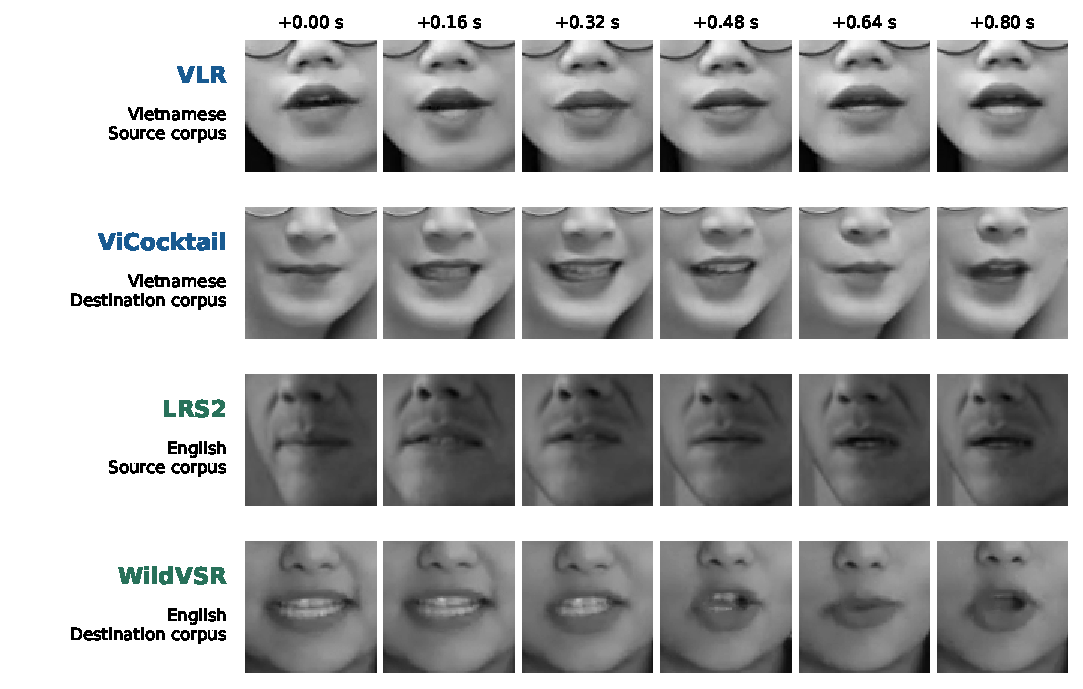
\includegraphics[width=\linewidth]{dataset_examples.pdf}
 \caption{Prepared mouth-region sequences from VLR~\cite{vlr2026dataset},
 ViCocktail~\cite{nguyen2025vicocktail}, LRS2~\cite{afouras2022deep} and
 WildVSR~\cite{djilali2024wildvsr}. Each row shows six real grayscale
 $88\times88$ center crops at 0.16-second intervals from one clip; displayed
 times are relative to the first illustrated frame. These examples show the
 visual input, while recognition is evaluated on complete clips.}
 \label{fig:datasets}
\end{figure}

A source-performance follow-up evaluates the initializer, FC and FM at seed 17
on all 11,307 prepared VLR test clips (225,960 reference units and 61 archived
source groups) and all 1,243 LRS2 test clips (6,660 words and 354 source groups).
Each corpus uses the same fitted states, preprocessing and frozen readouts as
its destination comparison. Source and destination results are analyzed
separately; the source follow-up does not add a second training seed.

\subsection{Continuation budget and controls}
All matched FC/FM comparisons use the final checkpoint after 6,000 updates, rather
than independently selected intermediate steps. The FM-ST and CP controls also
use step 6,000 and are evaluated at seed 17 in both corpus pairs. Training uses AdamW with peak
learning rate $2\times10^{-6}$, weight decay 0.01, 500 warm-up steps and cosine
decay. Eight individually processed examples are accumulated per optimizer step;
the gradient norm is clipped at 5. Training uses bfloat16 where supported, while
the assessment decoder uses float32. The same seed determines the source-clip
order and fragment choices across paired methods.

The fragment-eligibility rule requires 82--400 prepared frames, usable timing
and feasible target sequences. This has different consequences across corpora.
The Vietnamese matched runs draw 48,000 distinct clips from a pool of 90,519. The
English runs draw from 7,291 eligible clips, each revisited six or seven times.
Thus, both English FC and FM share the long-clip subset; FC does not receive the
short clips excluded from that matched comparison. An additional English full-pool
FC run (F0) uses the complete eligible full-clip pool of 45,838 clips at the same
6,000-update budget. It tests a practical alternative training population, rather
than isolating the crop transformation on identical examples.

We report the uncontinued initializer in each setting. We also report a native
ViCocktail model and the larger-data English Auto-AVSR model to indicate the
remaining performance gap. These practical references have different training
resources; the native ViCocktail system also has its own preprocessing. They are
not used to estimate the effect of FM relative to FC.

\subsection{Matched comparison of fragment labelling rules}
\label{sec:matchedcrop}
A follow-up VLR-to-ViCocktail experiment trains full-only, fixed-time and
whole-word continuations together in one training runtime at seed 17.
All three start from the same initializer and use the same 48,000 source-clip
presentations, 6,000 updates, optimizer schedule and native hybrid objective.
The two mixed arms share 317 full-clip fallback positions, yielding 24,317 full
and 23,683 short presentations per arm. They are newly fitted states, distinct
from the original FC/FM checkpoints. Their own source assessment covers all
11,307 VLR test clips under the same common decoder, with paired intervals
resampling the 61 source-video groups. Each new state is therefore assessed
on both source and destination without changing its weights or readout.

The crop rules in Section~\ref{sec:wordviews} and the final-update endpoint are
fixed before this follow-up's assessment. Its main comparison uses the common
decoder on the same 1,167 ViCocktail clips, without choosing a separate decoder
for each new model. This is a focused augmentation control on a previously used
assessment set, not a new independent corpus confirmation. Its conditional
intervals use the same 20 source groups and 10,000 paired resamples. We report
this comparison separately so that the shared fallbacks and fitted states are
not conflated with the original two-seed experiment.

A further pre-specified short-only state at seed 17 uses the schedule in
Section~\ref{sec:shortonly}; the three completed native states remain its fixed
comparators. Its assessment protocol covers the same 11,307 VLR source clips
and 1,167 ViCocktail destination clips, using the common decoder without a new
decoder search. The primary contrast is whole-word mixed minus short-only WER;
the reference contrast is full-only minus short-only WER. Positive differences
favor short-only supervision. Fixed-time mixing is a supporting comparison,
rather than an additional primary contrast. The two population-specific analyses
use 10,000 paired resamples of the 61 VLR or 20 ViCocktail archived source groups.
The plan and contrast directions were fixed before short-only training.
Intervals are conditional on these fitted states, pointwise and unadjusted for
multiplicity. No equivalence margin was specified, so an interval spanning zero
does not establish that mixing and short-only supervision are equivalent.
This follow-up also reuses previously observed assessment corpora and adds no
new training seed or independent test collection.

The loss-reduction control fits a further full-only/fixed-time pair using
Equation~\ref{eq:normalized}, with the same initializer, source schedules,
shared fallbacks, seed, optimizer and final-update endpoint as the matched crop
comparison. All four native/normalized states use the common decoder. We compute
the difference between their full-minus-fixed-time gains using paired resamples
of the same recording groups across all four states. No normalized whole-word
arm is included in this comparison.

\subsection{Decoder selection and metrics}
For the original FC/FM comparisons and same-target context controls, each
checkpoint's primary decoder is selected by aggregate error count on development
data from a fixed set of 11 candidates. The matched crop, short-only and
loss-reduction follow-ups use the common decoder without a new search. The candidates comprise hybrid
beam decoding with CTC weights $\alpha\in\{0.1,0.5,0.9,1.0\}$ and greedy CTC with
blank-logit biases $b\in\{0,-0.5,0.5,-1,1,-2,2\}$. Ties use a fixed candidate
order. Beam decoding uses width 40, zero length penalty and no external language
model. The search horizon covers the full encoded frame sequence. The common
decoder is the same beam decoder with $\alpha=0.1$ for all checkpoints.

Vietnamese primary selection uses 768 ViCocktail development clips, whereas
English selection uses 1,082 LRS2 source-development clips. Vietnamese therefore
allows target-domain decoder calibration without target-domain gradient updates;
English uses source-only decoder calibration. We do not treat these as identical
zero-shot protocols. The common-decoder comparison removes model-specific decoder
selection, although it cannot remove differences in the corpora or initializers.

Text is normalized with Unicode NFC, lowercasing and whitespace normalization.
We compute corpus-level WER as $100(S+D+I)/N$, where $N$ is the total reference
unit count. Vietnamese whitespace-delimited units need not coincide with lexical
words; consequently, its WER is not pooled with English WER. We report absolute
percentage-point differences and the underlying substitution, deletion and
insertion counts. Positive FC--FM differences favor FM.

Paired bootstrap intervals use 10,000 resamples. Vietnamese resampling preserves
the 20 original-video groups; WildVSR resampling uses released clips because a
validated recording-group reconstruction is unavailable. The WildVSR intervals are
therefore conditional clip-resampling summaries and do not establish uncertainty
over independent recording sources. The source follow-up resamples 61 VLR or
354 LRS2 archived source groups, which are not asserted to be verified speaker
identities. These resampling units differ across corpora. All intervals condition on the
fitted seeds and chosen decoders. For the mechanism comparison, FM--FM-ST and
FM--CP are the primary contrasts; comparisons with FC describe how much of the
original transfer gain remains. Intervals are pointwise, without adjustment for
multiple comparisons. The assessment sets have appeared in earlier
experiments; the results should therefore be interpreted as retrospective
evidence rather than confirmation on an untouched test set. The source-performance follow-up also uses previously observed test data.
Upstream training overlap is not independently established.
